% =====================================================================
%  Chapitre 3 -- partie b : regularisation
% =====================================================================

\begin{frame}{Quand la complexité se retourne contre nous}
\begin{columns}[t]
\begin{column}{0.52\textwidth}
\centering
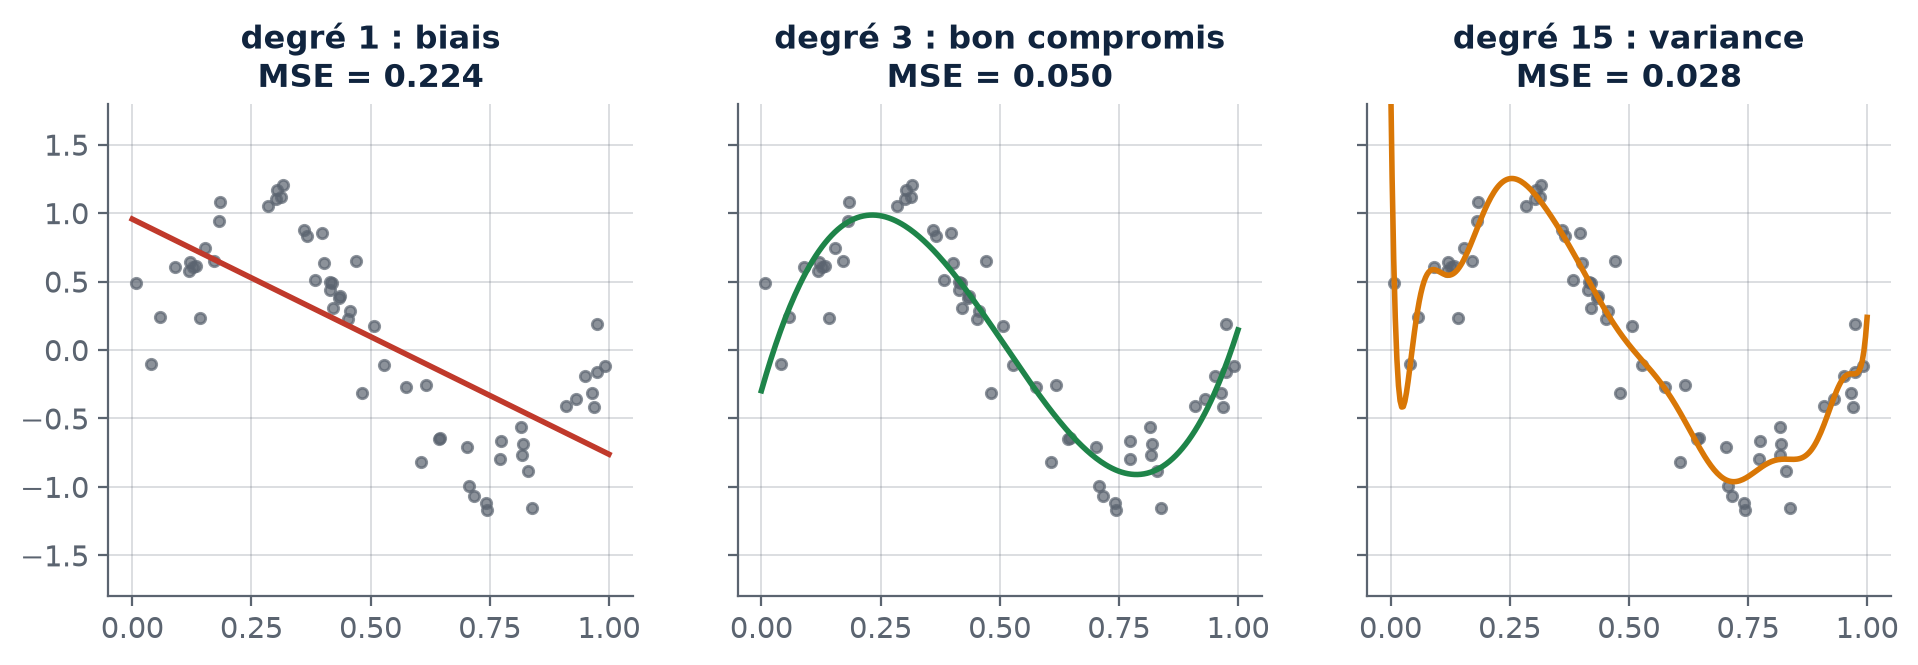
\includegraphics[height=0.32\textheight,keepaspectratio]{k02_polynomes.png}
\end{column}
\begin{column}{0.44\textwidth}
\begin{itemize}
  \item Degré 1 : MSE $=\mathbf{0{,}224}$ --- biais.
  \item Degré 3 : MSE $=\mathbf{0{,}050}$ --- bon compromis.
  \item Degré 15 : MSE $=\mathbf{0{,}028}$ sur l'entraînement, mais la courbe
        oscille entre les points.
\end{itemize}
\begin{wbox}[Le piège]
L'erreur d'entraînement ne cesse de baisser. C'est l'erreur sur des points
nouveaux qui se dégrade.
\end{wbox}
\end{column}
\end{columns}
\end{frame}

\begin{frame}{L'idée de la régularisation}
\begin{columns}[t]
\begin{column}{0.50\textwidth}
Ajouter à la perte une \textbf{pénalité} sur la taille des coefficients :
\[
  \hat{\boldsymbol\beta}
  =\argmin_{\boldsymbol\beta}\;
  \underbrace{\sum_{i}(y_i-\hat y_i)^2}_{\text{ajustement}}
  \;+\;
  \underbrace{\lambda\,\Omega(\boldsymbol\beta)}_{\text{pénalité}} .
\]
Plus $\lambda$ est grand, plus le modèle est contraint.
\end{column}
\begin{column}{0.46\textwidth}
\begin{kbox}[Ce que l'on échange]
On accepte un peu plus de \textbf{biais} pour réduire fortement la
\textbf{variance}. Le $\lambda$ optimal est celui qui minimise l'erreur de
validation, pas l'erreur d'entraînement.
\end{kbox}
\begin{wbox}[Pourquoi cela fonctionne]
Un coefficient très grand est le signe d'un modèle qui s'accroche au bruit :
le pénaliser l'empêche de le faire.
\end{wbox}
\end{column}
\end{columns}
\end{frame}

\begin{frame}{Ridge et Lasso : deux pénalités, deux effets}
\begin{center}
\small
\begin{tabular}{@{}p{0.14\textwidth}p{0.24\textwidth}p{0.26\textwidth}p{0.24\textwidth}@{}}
\toprule
\textbf{Méthode} & \textbf{Pénalité} & \textbf{Effet sur les coefficients} &
\textbf{Usage} \\
\midrule
Ridge & $\lambda\sum_j \beta_j^2$ & contraction douce, aucun ne s'annule &
variables corrélées, toutes utiles \\
Lasso & $\lambda\sum_j |\beta_j|$ & certains coefficients deviennent
\textbf{exactement nuls} & sélection de variables \\
ElasticNet & $\lambda\big(\alpha\sum|\beta_j|+(1-\alpha)\sum\beta_j^2\big)$ &
mélange des deux & variables corrélées et nombreuses \\
\bottomrule
\end{tabular}
\end{center}
\vspace{2mm}
\begin{kbox}[La différence tient à la forme de la pénalité]
La valeur absolue crée un « coin » en zéro : l'optimum s'y accroche. Le carré
contraint sans jamais annuler.
\end{kbox}
\end{frame}

\begin{frame}{Voir les chemins de régularisation}
\begin{center}
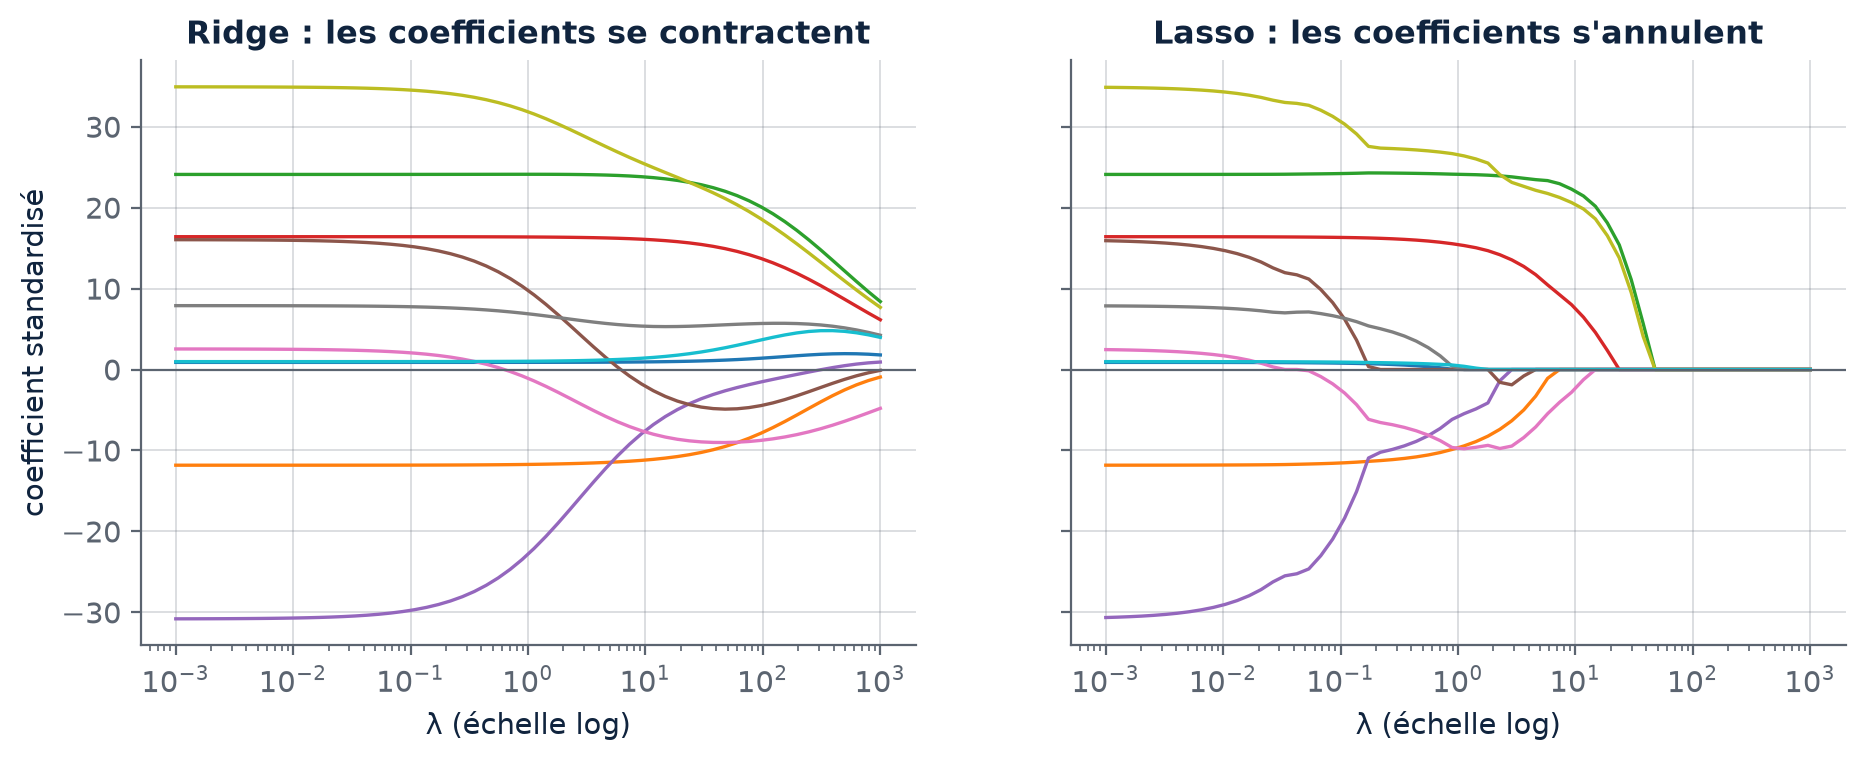
\includegraphics[width=0.95\textwidth]{k03_chemins.png}
\end{center}
\vspace{1mm}
\begin{columns}[t]
\begin{column}{0.48\textwidth}
\footnotesize
\textbf{Ridge} : toutes les courbes se rapprochent de zéro sans l'atteindre.
\end{column}
\begin{column}{0.48\textwidth}
\footnotesize
\textbf{Lasso} : les courbes touchent zéro l'une après l'autre. À
$\lambda$ maximal, les \textbf{10 coefficients} du jeu sont nuls.
\end{column}
\end{columns}
\end{frame}

\begin{frame}{Standardiser avant de pénaliser}
\begin{columns}[t]
\begin{column}{0.48\textwidth}
\begin{wbox}[Le problème]
La pénalité porte sur la \textbf{taille} des coefficients. Or cette taille dépend
de l'unité : un coefficient exprimé en « par FCFA » est minuscule, le même effet
en « par million de FCFA » est énorme.
\end{wbox}
\end{column}
\begin{column}{0.48\textwidth}
\begin{solbox}[La règle]
Standardiser \textbf{avant} la pénalité, et dans le \textbf{pipeline} : la
moyenne et l'écart-type sont estimés sur l'entraînement seulement.
\end{solbox}
\end{column}
\end{columns}
\vspace{2mm}
\begin{kbox}[Conséquence]
Sans standardisation, la régularisation ne pénalise pas la complexité : elle
pénalise arbitrairement les variables exprimées dans les plus petites unités.
\end{kbox}
\end{frame}

\begin{frame}{Mesurer la colinéarité : le VIF}
\begin{columns}[t]
\begin{column}{0.50\textwidth}
Pour chaque variable $j$, on régresse $x_j$ sur toutes les autres et on note
$R_j^2$ :
\[
  \mathrm{VIF}_j=\frac{1}{1-R_j^2}.
\]
\begin{itemize}
  \item VIF $=1$ : aucune colinéarité.
  \item VIF $>5$ : à surveiller.
  \item VIF $>10$ : problème sérieux.
\end{itemize}
\end{column}
\begin{column}{0.46\textwidth}
\begin{kbox}[Lecture]
Un VIF de 10 signifie que 90 \% de la variance de $x_j$ est déjà expliquée par
les autres variables : son coefficient n'apporte presque rien de propre.
\end{kbox}
\begin{wbox}[Remèdes]
Supprimer une des variables, les combiner (moyenne, ACP), ou régulariser avec
Ridge.
\end{wbox}
\end{column}
\end{columns}
\end{frame}

\begin{frame}{Comparer des coefficients : standardiser}
\begin{columns}[t]
\begin{column}{0.48\textwidth}
\begin{wbox}[Le problème]
Un coefficient de $0{,}002$ sur un revenu en FCFA peut être cent fois plus
décisif qu'un coefficient de $2$ sur un âge en années.
\end{wbox}
\end{column}
\begin{column}{0.48\textwidth}
\begin{solbox}[La solution]
Standardiser les variables : les coefficients s'expriment alors en « écart-type
de $y$ par écart-type de $x$ » et deviennent comparables.
\end{solbox}
\end{column}
\end{columns}
\vspace{2mm}
\begin{kbox}[Ce que cela ne change pas]
La prédiction est identique : seule la \textbf{lecture} des coefficients change.
Standardiser ne rend pas un modèle meilleur, seulement plus lisible.
\end{kbox}
\end{frame}

\begin{frame}{Choisir $\lambda$}
\begin{center}
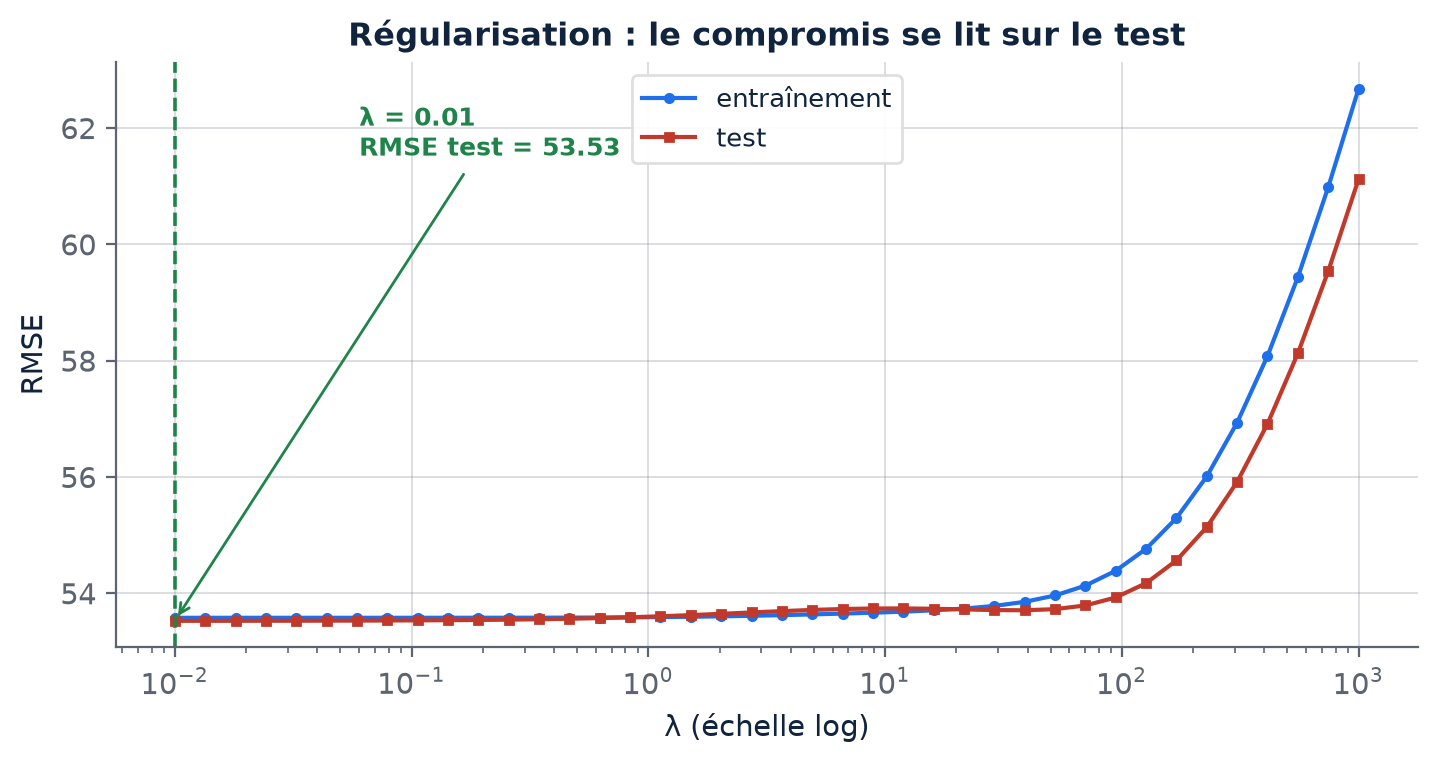
\includegraphics[width=0.54\textwidth]{k04_lambda.png}
\end{center}
\vspace{-1mm}
\begin{columns}[t]
\begin{column}{0.46\textwidth}
\footnotesize
\begin{itemize}
  \item $\lambda$ trop petit : même erreur que l'OLS.
  \item $\lambda$ trop grand : sous-apprentissage (RMSE $61{,}1$).
  \item Ici la courbe de test est \textbf{plate} : l'erreur varie à peine.
\end{itemize}
\end{column}
\begin{column}{0.50\textwidth}
\begin{wbox}[Ce que fait la validation croisée]
Elle retient $\lambda\approx\mathbf{29}$ ; le test donne $53{,}7$ contre
$53{,}5$ pour l'OLS : \textbf{aucun gain}.
\end{wbox}
\end{column}
\end{columns}
\end{frame}

\begin{frame}{Où la régularisation change tout}
\begin{columns}[t]
\begin{column}{0.46\textwidth}
\centering
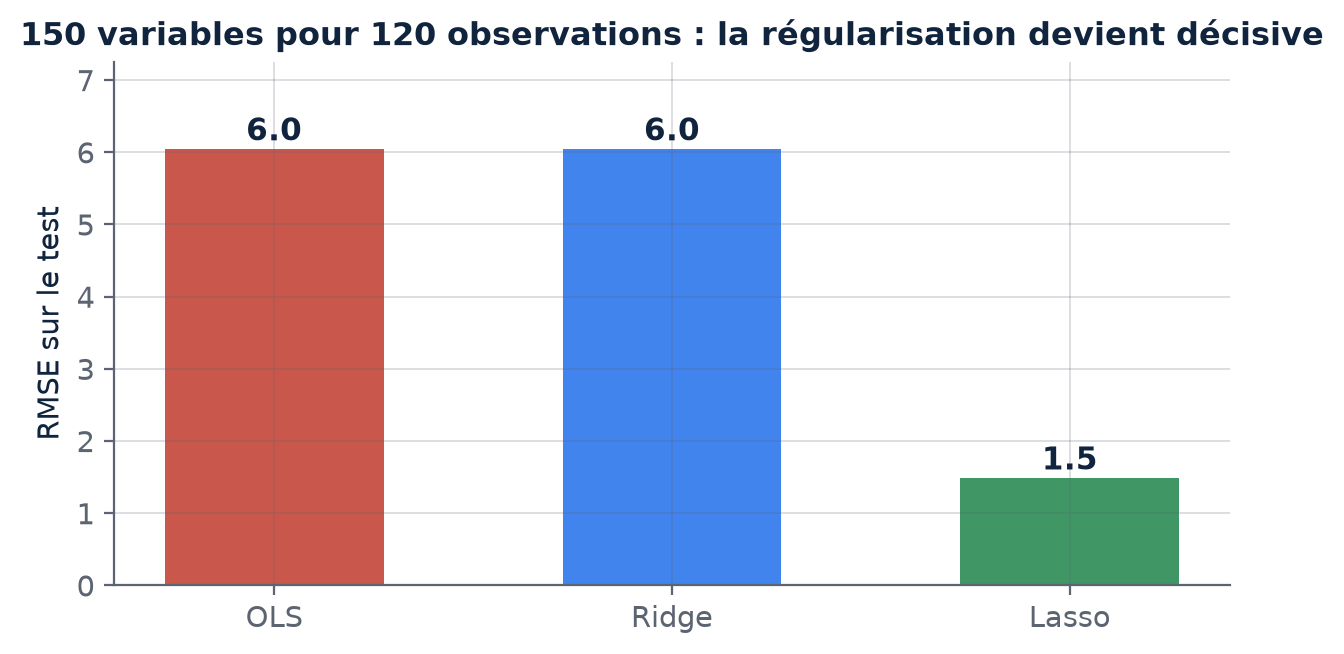
\includegraphics[height=0.32\textheight,keepaspectratio]{k09_grande_dimension.png}
\end{column}
\begin{column}{0.52\textwidth}
\begin{itemize}
  \item 150 variables pour 120 observations, dont \textbf{8 informatives}.
  \item OLS : RMSE $\mathbf{6{,}04}$.
  \item Ridge : $\mathbf{6{,}04}$ --- sans effet ici.
  \item Lasso : $\mathbf{1{,}48}$ --- l'erreur est divisée par 4.
\end{itemize}
\begin{solbox}[Pourquoi]
Le Lasso retient \textbf{11 coefficients non nuls}, dont les \textbf{8 vraies
variables}. Il sélectionne au lieu de contracter.
\end{solbox}
\end{column}
\end{columns}
\end{frame}

\begin{frame}{Comparaison honnête sur le jeu du diabète}
\begin{columns}[t]
\begin{column}{0.42\textwidth}
\centering
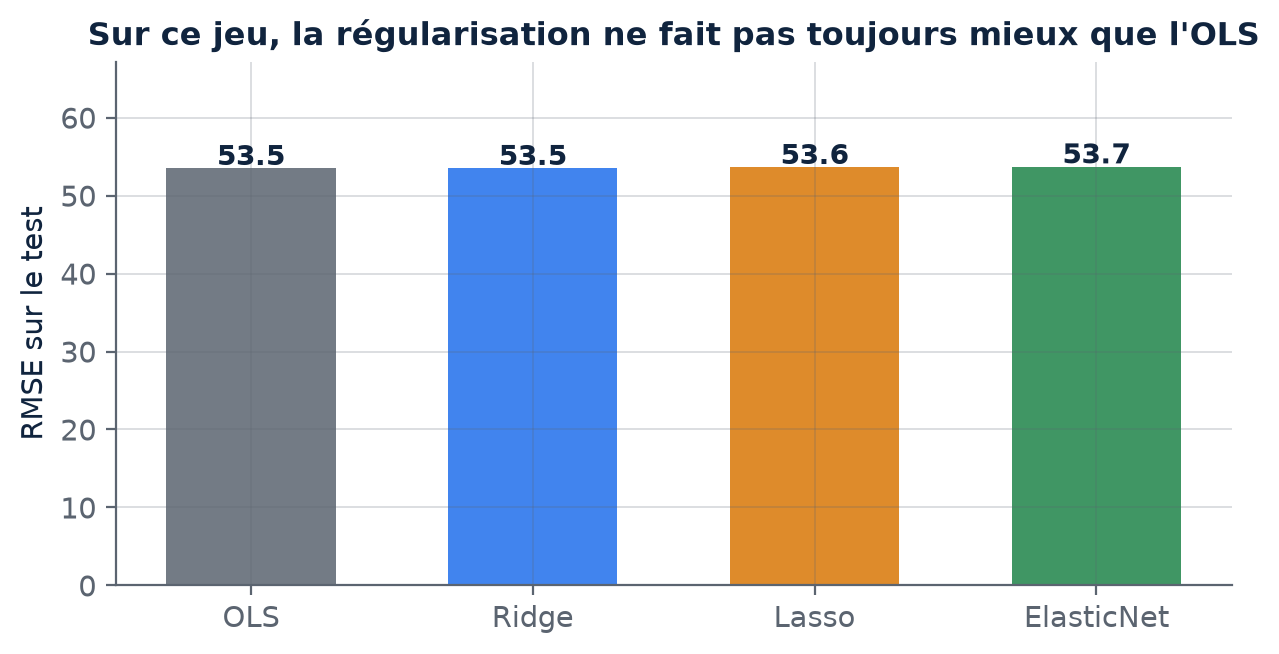
\includegraphics[height=0.32\textheight,keepaspectratio]{k08_comparaison.png}
\end{column}
\begin{column}{0.54\textwidth}
\begin{center}
\small
\begin{tabular}{@{}lr@{}}
\toprule
\textbf{Modèle} & \textbf{RMSE test} \\
\midrule
OLS & $\mathbf{53{,}52}$ \\
Ridge & $53{,}53$ \\
Lasso & $53{,}65$ \\
ElasticNet & $53{,}73$ \\
\bottomrule
\end{tabular}
\end{center}
\begin{wbox}[Ce que cela enseigne]
Avec 10 variables et 331 observations, l'OLS n'a pas besoin d'aide. La
régularisation est un outil pour la \textbf{grande dimension} ou la
\textbf{colinéarité}, pas un réflexe.
\end{wbox}
\end{column}
\end{columns}
\end{frame}

\begin{frame}{Activité 2 --- choisir la pénalité (8 min)}
\begin{abox}[Trois situations]
\begin{enumerate}
  \item 500 variables, 80 observations, vous soupçonnez que 20 comptent.
  \item 30 variables très corrélées entre elles (mesures répétées).
  \item 10 variables bien choisies, 5\,000 observations.
\end{enumerate}
Quelle pénalité, et pourquoi ?
\end{abox}
\vspace{1mm}
\begin{solbox}[Réponses]
\textbf{1.} Lasso : sélection nécessaire.
\textbf{2.} Ridge, ou ElasticNet si le Lasso élimine trop brutalement.
\textbf{3.} Aucune : l'OLS est adapté, la régularisation n'apportera rien.
\end{solbox}
\end{frame}

\begin{frame}{Quiz 2 --- régularisation}
\begin{columns}[t]
\begin{column}{0.49\textwidth}
\begin{qbox}[Question 1]
Quelle pénalité annule exactement des coefficients ?
\begin{itemize}
  \item[(a)] Ridge \quad (b) Lasso \quad (c) les deux
\end{itemize}
\end{qbox}
\begin{qbox}[Question 2]
$\lambda$ se choisit sur :
\begin{itemize}
  \item[(a)] l'erreur d'entraînement
  \item[(b)] la validation croisée
  \item[(c)] le test, une fois
\end{itemize}
\end{qbox}
\end{column}
\begin{column}{0.49\textwidth}
\begin{qbox}[Question 3]
Avant une pénalité, il faut :
\begin{itemize}
  \item[(a)] standardiser \quad (b) normaliser $y$
  \item[(c)] rien de particulier
\end{itemize}
\end{qbox}
\begin{solbox}[Réponses]
\textbf{1.} (b). \quad \textbf{2.} (b) : on ne touche pas au test.
\quad \textbf{3.} (a).
\end{solbox}
\end{column}
\end{columns}
\end{frame}
